%!TeX root=../tese.tex

%% ------------------------------------------------------------------------- %%
\chapter{Proposta de trabalho}
\label{cap:proposta-de-trabalho}

Inicialmente partiremos de registros de requisições processadas por uma aplicação
de teste para detectar e analisar anomalias que tenham acontecido durante o tempo
em que os registros foram coletados. Posteriormente, será implementado um modelo
onde esta análise ocorrerá de forma contínua, com um período de aprendizado no
início seguido do aprimoramento constante conforme a aplicação é utilizada.

Para a avaliação da aplicação de teste as seguintes etapas serão necessárias:

\begin{enumerate}
  \item Coleta de registros de requisições;
  \item Filtragem dos registros de requisições;
  \item Agregação de registros e extração de novas características;
  \item Avaliação da URL acessada;
  \item Treinamento dos modelos;
  \item Detecção de caso anômalo;
  \item Avaliação de melhoria contínua do treinamento inicial;
  \item Classificação de caso anômalo;
  \item Agregação de casos anômalos classificados.
\end{enumerate}

\section{Etapa 1 - Coleta de registros de requisições}
\label{sec:etapa-1}

Os registros das requisições processadas serão extraídos a partir de balanceadores
de carga conforme o diagrama abaixo sem adicionar complexidade ou atraso na resposta
do serviço uma vez que os balanceadores de carga já são elementos necessários para
garantir a alta disponibilidade de uma aplicação web.

\begin{figure}
  \centering
  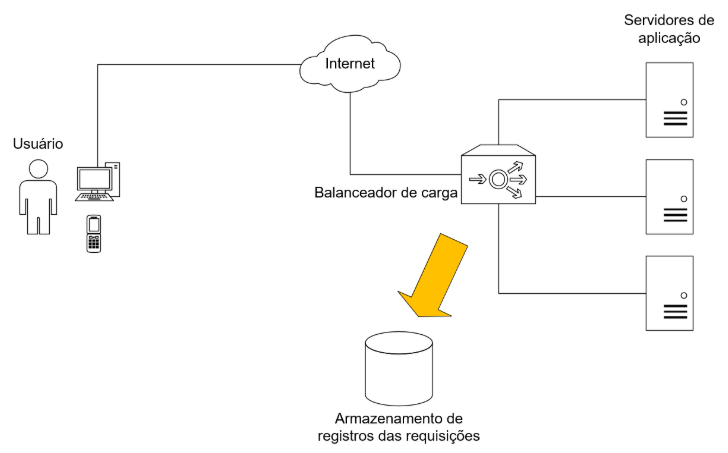
\includegraphics[width=.7\textwidth]{figura6}
  \caption{Extração de dados de balanceadores de carga.\label{fig:extracao-de-dados-de-balanceadores-de-carga}}
\end{figure}

Existem muitas opções de balanceadores de carga possíveis, entretanto as informações
abaixo relacionadas estão presentes nas principais aplicações ou serviços utilizados
como balanceadores de carga (por exemplo: Nginx\footnote[8]{\url{http://www.nginx.com}},
HA-Proxy\footnote[9]{http://www.haproxy.org}, AWS Application Load 
Balancer\footnote[10]{http://aws.amazon.com/elasticloadbalancing}):

\begin{itemize}
  \item Data e hora da solicitação;
  \item URL solicitada;
  \item Verbo HTTP utilizado;
  \item Instância/máquina que realizou o processamento;
  \item Quantidade de bytes recebidos;
  \item Quantidade de bytes enviados;
  \item Tempo de processamento;
  \item Código de resposta HTTP.
\end{itemize}

Como cada balanceador de carga tem seu formato de registro de uma requisição
intermediada, estes registros serão convertidos em um formato padrão que será
utilizado pelas etapas seguintes.

\section{Etapa 2 - Filtragem dos registros de requisições}
\label{sec:etapa-2}

Esta etapa é necessária para filtrar eventuais registros indesejados dos
balanceadores de carga pois eventualmente o balanceador de carga pode ser
responsável por mais de uma aplicação web, e seus registros podem conter
dados que não desejamos tratar.

Também existem registros de falhas indeterminadas, ou com ausência das
informações apontadas na etapa 1, que desejamos remover para evitar ruídos
nos dados.

O caso específico de falha na comunicação entre o balanceador de carga e a
aplicação deverá ter o código de resposta HTTP mapeado para zero para que
este cenário importante possa ser detectado, pois pode sinalizar falhas em
uma instância.

\section{Etapa 3 - Agregação e extração de características dos registros
         para o aprendizado de máquina}
\label{sec:etapa-3}

Nesta etapa será extraída a informação de taxa de requisições concorrentes,
que não fazem parte de um registro isolado, mas dependem de um conjunto de
registros que estavam sendo processados no mesmo espaço de tempo.

Tomando uma janela de tempo fixa, ou de acordo com o tempo que a requisição
levou para ser processada, podemos recuperar a taxa de requisições a qual a
aplicação web estava sendo submetida.

Para o cálculo deste valor será utilizado como identificador somente a
identificação da instância que processou a requisição, independente de verbo
HTTP e URL, uma vez que desejamos saber a taxa de requisições concorrentes da
instância e não de uma requisição específica.

A mesma abordagem pode ser utilizada para o tráfego de dados para tentar
identificar que o gargalo na execução de uma requisição são as interfaces de
comunicação com a rede, porém por não ser certo que os bytes trafegados foram
distribuídos uniformemente durante o intervalo de tempo da requisição esta
métrica será deixada de lado neste momento.
 
Para a recuperação da taxa de requisições concorrentes será implementado um
contador de requisições ativas para cada janela de 1 segundo, e durante o
intervalo de tempo em que a requisição esteve ativa os contadores serão
incrementados. O intervalo de 1 segundo é o que se espera ser o mais adequado,
entretanto durante a execução da pesquisa será avaliado se este valor é de
fato o mais adequado.

\begin{figure}
  \centering
  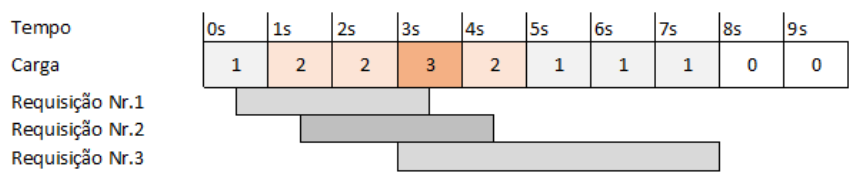
\includegraphics[width=.8\textwidth]{figura7}
  \caption{Carga de requisições ao longo do tempo.\label{fig:carga-de-requisicoes-ao-longo-do-tempo}}
\end{figure}

Adicionalmente serão extraídas novas características para o valor de resposta
HTTP dado que um modelo de aprendizado de máquina não conseguiria estabelecer
uma relação linear para os códigos de retorno. Para isto serão isolados em
características distintas e mapeados de acordo com a tabela abaixo:

\begin{table}[H]
\centering
\caption{Mapeamento de respostas HTTP para um vetor.}
\vspace{0.25cm}
\begin{tabular}{ll}
Resposta HTTP & Vetor de características            \\
\hline
0	      &	[0, 0, 0, 0, 0]                         \\
100 a 199 &	[1000, 0, 0, 0, 0] a [1099, 0, 0, 0, 0] \\
200 a 299 &	[0, 1000, 0, 0, 0] a [0, 1099, 0, 0, 0] \\
300 a 399 &	[0, 0, 1000, 0, 0] a [0, 0, 1099, 0, 0] \\
400 a 499 &	[0, 0, 0, 1000, 0] a [0, 0, 0, 1099, 0] \\
500 a 599 & [0, 0, 0, 0, 1000] a [0, 0, 0, 0, 1099]
\end{tabular}
\end{table}

Acima estão sendo utilizados os valores de dois parâmetros que serão ajustados
posteriormente de acordo com os resultados dos testes. São estes:

\begin{table}[H]
\caption{Parâmetro $H_{min}$.}
\vspace{0.25cm}
\begin{tabular}{ll}
Parâmetro      & $H_{min}$ \\
Valor proposto & 1000 \\
Descrição      & Valor mínimo caso a categoria de respostas HTTP esteja ativa.
\end{tabular}
\end{table}

\begin{table}[H]
\caption{Parâmetro $H_{range}$.}
\vspace{0.25cm}
\begin{tabular}{ll}
Parâmetro      & $H_{range}$ \\
Valor proposto & 100 \\
Descrição      & Valor para o qual os valores da categoria X, de X00 a X99 deverão \\
               & ter sua escala ajustada.
\end{tabular}
\end{table}

Ou seja, o vetor de características $R_{vector}$ para um código de resposta R poderia ser gerado com:

\begin{program}
  \centering
  \begin{lstlisting}[language=Java, style=wider]
    int[] getRVector(int R, int hMin, int hRange) {
        int[] rVector = new int[] { 0, 0, 0, 0, 0 };
        if (R > 100) {
            rVector[ (int) Math.floor( R / 100 ) - 1 ] = hMin + (int) ((float) (R \% 100) / 100 * hRange);
        }
	    return rVector;
	}
  \end{lstlisting}
  \caption{Código para cálculo do vetor $R_{vector}$.\label{prog:java}}
\end{program}

Os valores 1000 e 100 estão sendo utilizados para que o valor 0, que representa
a não ocorrência daquela característica, esteja suficientemente distante e que
permita ainda as variações dentre a categoria de resposta serem detectadas.
O valor 0 que representa ausência de resposta HTTP está sendo mapeado para um
vetor zero que difere bastante dos outros valores em caso de resposta.

Posteriormente será avaliada a necessidade de normalizar as características
coletadas para que a detecção seja mais eficiente, porém neste momento da
pesquisa esta etapa aparenta não ser necessária.

Também será analisada a ideia de se isolar códigos de erro específicos que
indiquem algum cenário, como por exemplo:

\begin{itemize}
  \item 401 (Unauthorized) e 403 (Forbidden): Indicam falhas relacionadas a permissão de acesso;
  \item 502 (Bad Gateway) e 504 (Gateway timeout): Indicam possíveis falhas com serviços do qual a aplicação depende.
\end{itemize}

\section{Etapa 4 - Avaliação da URL acessada}
\label{sec:etapa-4}

Esta etapa determina como a URL será utilizada para ter seus registros agrupados
em uma forma que seja possível determinar quais URLs correspondem a um determinado
serviço da aplicação web.

Existe um problema crítico na utilização da uma URL para identificar um tipo de
serviço, visto que identificadores de recursos são bastante comuns em parte do
caminho acessado. Por exemplo, em uma aplicação de cuida de cadastros de clientes
pode ter requisições como as abaixo:

\begin{table}[H]
\centering
\caption{Exemplos de requisições HTTP.}
\vspace{0.25cm}
\begin{tabular}{ll}
Verbo & Caminho do recurso \\
\hline
POST & /clientes           \\
GET  & /clientes/42        \\
PUT  & /clientes/42        \\
GET  & /clientes/99        \\
GET  & /clientes/999       \\
GET  & /health
\end{tabular}
\end{table}

Das requisições acima relacionadas, as de verbo ``GET'' para o caminho
``/clientes/\{número\}'' são bastante parecidas e provavelmente devem executar um
código de recuperação de dados do cliente identificado pelo número.

Para agrupar estes dados será utilizada uma estrutura de árvore com os caminhos
acessados e os nós mais ``comuns'' terão uma quantidade de registros maior que os
demais.

\begin{figure}
  \centering
  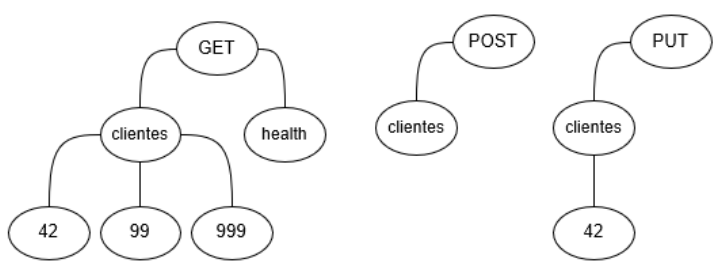
\includegraphics[width=.7\textwidth]{figura8}
  \caption{Caminho da URL em uma árvore.\label{fig:caminho-da-url-em-uma-arvore}}
\end{figure}

Ao receber um registro de uma requisição a árvore será percorrida e os nós que
fazem parte do caminho deste registo terão uma referência para este registro,
desta forma será possível avaliar quais são os nós que tem relevância para agrupar
registros por um número suficientemente grande de referências, porém com nós filhos
com poucas referências.

Será avaliada também a ideia de utilizar expressões regulares para definir os
serviços monitorados, pois em alguns cenários a utilização do caminho inicial comum
pode não ser suficiente para identificar o grupo de requisições.

\section{Etapa 5 - Treinamento dos modelos}
\label{sec:etapa-5}

Uma vez que as etapas anteriores já coletaram e processaram os dados das requisições,
o treinamento dos modelos poderá ser iniciado. Caso existam dados salvos de
treinamentos anteriores, eles poderão ser carregados para serem aprimorados com
novos registros.

O treinamento será independente para cada conjunto de verbo HTTP, caminho parcial da
URL e instância monitorada, conforme descrito na etapa 4, desta forma estaremos
monitorando sempre o mesmo código executado da aplicação web apesar de que sua
execução poderá ser diferente de acordo com os parâmetros.

Dado que estamos considerando a instância monitorada, também será possível na etapa
de classificação identificar se as anomalias acontecem em algumas instâncias somente. 

Durante o desenvolvimento desta pesquisa serão avaliados diversos parâmetros que
poderão ser alterados conforme a necessidade. Inclusive descobrir quais parâmetros
deverão ser alterados e para que valores é parte do desafio de pesquisa. São estes:

\begin{table}[H]
\caption{Parâmetro $N_{min}$.}
\vspace{0.25cm}
\begin{tabular}{ll}
Parâmetro      & $N_{min}$ \\
Valor proposto & 1000 \\
Descrição      & Número mínimo de registros que deverão ser utilizados no \\
               & treinamento de um modelo.
\end{tabular}
\end{table}

\begin{table}[H]
\caption{Parâmetro $T_{min}$.}
\vspace{0.25cm}
\begin{tabular}{ll}
Parâmetro      & $T_{min}$ \\
Valor proposto & 86400 \\
Descrição      & Tempo mínimo em segundos que as requisições devem ser \\
               & coletadas para um treinamento sem dados prévios.
\end{tabular}
\end{table}

A etapa de detecção de anomalias irá se basear em avaliação de probabilidade em uma
distribuição multivalorada gaussiana (mais informações em \citep{ng}), que será
treinada uma vez que ambos os critérios de $N_{min}$ e $T_{min}$ sejam obedecidos.

Assim que houver a quantidade de amostras necessária, as fórmulas abaixo serão
aplicadas para $m$ registros $x_i$ e os valores de $\mu$ e $\Sigma$ corresponderão ao
treinamento para estes registros.

\begingroup
\Large
\begin{equation}
\displaystyle \mu = \frac{1}{m} \sum_{i=1}^{m} x_i , \mu \in \mathbb{R}^d
\end{equation}
\endgroup

\begingroup
\Large
\begin{equation}
\displaystyle \Sigma = \frac{1}{m} \sum_{i=1}^{m} \left[ ( x_i - \mu ) ( x_i - \mu )^{T} \right] , \Sigma \in \mathbb{R}^{d \times d}
\end{equation}
\endgroup

\section{Etapa 6 - Detecção de caso anômalo}
\label{sec:etapa-6}

Para a detecção de caso anômalo será calculada a probabilidade $p(x_i)$ de um caso $x_i$
ser semelhante aos casos observados no cálculo de $\mu$ e $\Sigma$, e o valor limite será
definido através do parâmetro $P_{min}$.

\begin{table}[H]
\caption{Parâmetro $P_{min}$.}
\vspace{0.25cm}
\begin{tabular}{ll}
Parâmetro      & $P_{min}$ \\
Valor proposto & 0.25 \\
Descrição      & Probabilidade mínima requerida para que o registro sob análise \\
               & não seja considerado anômalo.
\end{tabular}
\end{table}

Caso a probabilidade $p(x_i)$ seja menor que $P_{min}$ a ocorrência $x_i$ será
classificada como anômala e passará pela etapa de classificação (etapa 8).

\begingroup
\Large
\begin{equation}
p(x_i; \mu, \Sigma) = \frac{1}{(2 \pi)^{\frac{n}{2}} | \Sigma |^{\frac{1}{2}} } exp \left( - \frac{1}{2} ( x_i - \mu )^{T} \Sigma^{-1} ( x_i - \mu ) \right)
\end{equation}
\endgroup

\section{Etapa 7 - Melhoria contínua do treinamento inicial}
\label{sec:etapa-7}

O treinamento inicial será realizado assim que houver a quantidade mínima de
registros necessários, entretanto após este treinamento inicial ser realizado,
o modelo definido por $\mu$ e $\Sigma$ deverá ser atualizado de regularmente
com todos os novos registros observados, tenham estes sido classificados como
anômalos ou não.

\begin{table}[H]
\caption{Parâmetro $T_{update}$.}
\vspace{0.25cm}
\begin{tabular}{ll}
Parâmetro      & $T_{update}$ \\
Valor proposto & 1800 \\
Descrição      & Tempo mínimo em segundos para que novos registros sejam considerados \\
               & no novo treinamento do modelo.
\end{tabular}
\end{table}

\begin{table}[H]
\caption{Parâmetro $P_{update}$.}
\vspace{0.25cm}
\begin{tabular}{ll}
Parâmetro      & $P_{update}$ \\
Valor proposto & 0.02 \\
Descrição      & Percentual em que os novos registros irão influenciar um modelo \\
               & treinado.
\end{tabular}
\end{table}

De forma paralela a detecção, um algoritmo de atualização será executado a
cada $T_{update}$ segundos para atualização dos valores $\mu$ e $\Sigma$ com $n$
novas amostras coletadas. As fórmulas utilizadas na etapa 5 serão alteradas de
forma que os novos registros tenham um peso limitado sobre os valores de $\mu$
e $\Sigma$ atuais, conforme abaixo:

\begingroup
\Large
\begin{equation}
\displaystyle \mu ' = (1 - P_{update} ) \mu + P_{update} \frac{1}{n} \sum_{i=1}^{n} x_i
\end{equation}
\endgroup

\begingroup
\Large
\begin{equation}
\displaystyle \Sigma ' = (1 - P_{update} ) \Sigma + P_{update} \frac{1}{n} \sum_{i=1}^{n} \left[ ( x_i - \mu ' ) ( x_i - \mu ' )^{T} \right]
\end{equation}
\endgroup

A importância de se limitar o quanto os novos registros irão afetar o treinamento
é de impedir que uma falha que dure vários minutos possa influenciar no
aprendizado de forma que estas falhas deixem de ser detectadas. Adicionalmente
também é importante limitar a influência de registros antigos para que mudanças
na aplicação possam influenciar o treinamento existente.

\section{Etapa 8 - Classificação de caso anômalo}
\label{sec:etapa-8}

Para a classificação do caso anômalo será utilizado o valor de $\delta_i = ( x_i - \mu )$
como dado de entrada pois ele representa o quanto cada característica diferiu do valor
médio esperado para ela.

Os vetores $\delta_i$ serão eventualmente pré-processados para normalizar os valores e
utilizando um algoritmo de regressão logística (mais informações em \citep{mostafa}),
ou outro mecanismo de aprendizado de máquina supervisionado, serão classificados como
algum dos tipos de falha abaixo:

\begin{itemize}
  \item Aplicação sobrecarregada;
  \item Aplicação sobrecarregada e irresponsiva;
  \item Falha em dependência da aplicação.
\end{itemize}

Dado que a ocorrência de falhas nas aplicações web não é algo frequente, serão
simulados alguns cenários com uma aplicação de teste para realizar o treinamento
deste modelo de aprendizado de máquina. A aplicação de teste será submetida aos
seguintes cenários:

\begin{enumerate}
  \item Aumento de carga além do esperado provocando um aumento no tempo de
        resposta mas sem gerar erros. Os resultados anômalos detectados serão
		classificados como ``Aplicação sobrecarregada'';
  \item Aumento de carga além do esperado provocando um aumento no tempo de
        resposta gerando erros, ou vindos da aplicação ou do balanceador de carga.
		Os resultados anômalos detectados serão classificados como ``Aplicação
		sobrecarregada e irresponsiva'';
  \item Remoção de dependência, como um banco de dados, provocando erros na resposta
        da aplicação. Os resultados anômalos serão classificados como ``Falha em
		dependência da aplicação''.
\end{enumerate}


\section{Etapa 9 - Agregação de casos anômalos classificados}
\label{sec:etapa-9}

Uma vez que as anomalias forem classificadas, será necessário avaliar a quantidade
de anomalias, para avaliar casos isolados, se elas foram classificadas da mesma
forma ou se são classificações variadas e ainda se é uma única instância que está
sofrendo desta anomalia ou várias delas.

Os resultados previstos a serem reportados são:

\begin{itemize}
  \item Nenhuma anomalia
  \item Pequenas anomalias detectadas
  \item Instância defeituosa
  \item Aplicação sobrecarregada
  \item Aplicação sobrecarregada e irresponsiva
  \item Falha em dependência da aplicação
  \item Falha geral na aplicação.
\end{itemize}

O parâmetro $A_{min}$ será utilizado para definir se o resultado final da análise
será de ``Pequenas anomalias detectadas'', indicando que algo anormal foi detectado
mas não tem relevância suficiente para disparar algum alarme ou ação automática.
Abaixo segue a definição deste parâmetro:

\begin{table}[H]
\caption{Parâmetro $A_{min}$.}
\vspace{0.25cm}
\begin{tabular}{ll}
Parâmetro      & $A_{min}$ \\
Valor proposto & 0.01 \\
Descrição      & Percentual mínimo de requisições anômalas para \\
               & que estas sejam apontadas.
\end{tabular}
\end{table}

Uma vez que a quantidade de anomalias sejam significantes deverá ser avaliado se
somente uma instância está sendo afetada. Em caso positivo o resultado final da
análise será de ``Instância defeituosa''.

Caso múltiplas instâncias sejam afetadas o resultado final da análise será dado
pela classificação que tenha mais de 50\% das ocorrências e caso não exista uma
que possua esta quantidade o resultado reportado deverá ser de ``Falha geral na
aplicação''. Este percentual inicialmente não será parametrizado, porém conforme
resultados da pesquisa ele poderá ser alterado.
